\section{设备管理}

\begin{frame}[fragile]{CH5 设备管理}
  \begin{easylist} \easyitem
    & 5.0 引言
    & 5.1 I/O系统的硬件组成
    & 5.2 I/O控制方式
    & 5.3 缓冲管理
    & 5.4 设备分配
    & 5.5 设备处理
    & 5.6 磁盘存储器管理
  \end{easylist}
\end{frame}


\subsection{引言}
\begin{frame}[fragile]{问题}
  \begin{easylist}
    & 设备管理的主要目标是什么?
    & 对应的主要解决途径是什么?
  \end{easylist}
\end{frame}

\begin{frame}[fragile]{引言}
  \begin{easylist}
    & “设备”泛指计算机系统中的外部设备,即除主机以外的其他所有设备。在多道程序设
    计环境下,计算机系统允许多个用户作业同时在内存,它们的运行势必涉及到I/O设备。
    & 带来三个问题 \pause
    && 对于设备本身,如何有效利用的问题;
    && 对于设备和CPU,如何发挥并行工作能力的问题;
    && 对于设备和用户,有一个如何方便使用的问题。
  \end{easylist}
\end{frame}

\begin{frame}[fragile]{引言}
  \begin{easylist}
    & 设备无关性
    && 操作系统必须向设备发送命令,捕捉中断,并处理设备的各种错误,还应提供其他
    部分使用设备的简单接口,如有可能,这个接口对所有设备都相同,这就是所谓的“与
    设备无关性”。
    & 虚拟设备
    && 在众多的I/O设备中,并不是所有的设备都是可以共享使用的。也就是说,当一个作
    业使用某种设备时,另一个要使用的作业只能暂时等待,一直到对方使用完毕,它才能
    去使用,这影响了系统效率的发挥。在设备管理中,仍然可以借助于磁盘,把只能独享
    的设备变为共享,这就是所谓的“虚拟设备”
  \end{easylist}
\end{frame}

\begin{frame}[fragile]{引言:设备管理的功能}
  \begin{easylist}
    & 缓冲区管理
    & 设备分配
    & 设备处理
    & 虚拟设备
    & 设备独立性
  \end{easylist}
\end{frame}

\begin{frame}[fragile]{通用设备管理分层模型}
  \begin{easylist}
    & 现代操作系统都采用分层结构构建设备管理模型,一种常见的设备管理模型如图
  \end{easylist}
  \begin{center} 
    \scalebox{0.8}{
      \begin{tikzpicture}[c/.style={draw,thick, minimum width=3cm, minimum height=0.75cm}, a/.style={<->, very thick}]
        \draw[] node[c] (b1) {用户进程} 
        node[c, below=0.5 of b1] (b2) {设备硬件无关层}
        node[c, below=0.5 of b2] (b3) {设备硬件相关层}
        node[c, below=0.5 of b3] (b4) {设备硬件} ;
        \draw[a] (b1)--(b2);
        \draw[a] (b2)--(b3);
        \draw[a] (b3)--(b4);
        \scriptsize
        \draw[] node[align=center,shape=ellipse, dotted, draw, fill=gray!5, minimum height=1cm,inner sep=0.1cm, left=0.5 of b3] (tip1) {实现\\I/O缓冲区管理\\以及\\设备映射功能};
        \draw[] node[align=center,shape=ellipse, dotted, draw, fill=gray!5, minimum height=1cm,inner sep=0cm, right=0.5cm of b2] (tip2) {将设备硬件无关层与硬件设备隔离开来。\\ 从设备硬件无关层看,设备硬件相关层为\\其提供了一个相对简洁的I/O功能接口;\\该接口屏蔽了设备硬件复杂的操作细节。\\从设备硬件相关层内部看,\\该层主要实现了设备驱动功能
        };
        \draw[->] (tip1)--(b2.west);
        \draw[->] (tip2)--(b3.east);
      \end{tikzpicture}
    }
  \end{center}
\end{frame}


\subsection{5.1 I/O系统的硬件组成}
\begin{frame}[fragile]{5.1 I/O系统的硬件组成}
  \begin{easylist}
    & 5.1.1 IO设备
    & 5.1.2 设备控制器
    & 5.1.3 IO通道
    & 5.1.4 总线系统
  \end{easylist}
\end{frame}

\subsubsection{5.1.1 IO设备}
\begin{frame}[fragile]{5.1.1 IO设备}
  \begin{enumerate}
    \item IO设备的类型
    \item 设备与控制器之间的接口
  \end{enumerate}
\end{frame}

\begin{frame}[fragile, allowframebreaks]{I/O设备的类型}
  \begin{easylist}
    & (1)按速度分:
    && 低速设备:典型设备有键盘、 鼠标器、语音的输入和输出等设备
    && 中速设备:典型设备有行式打印机、激光打印机等
    && 高速设备:典型设备有磁带机、 磁盘机、 光盘机等
    & (2)按信息交换的单位分类
    && 块设备(Block Device):用于存储信息,属于有结构设备。典型的块设备是磁盘。
    磁盘设备的基本特征是其传输速率较高,另一特征是可寻址,即对它可随机地读/写任
    一块;此外,磁盘设备的I/O常采用DMA方式
    && 字符设备(Character Device):用于数据的输入和输出,属于无结构设备。典型字
    符设备如交互式终端、打印机等。基本特征是其传输速率较低,另一特征是不可寻址;
    此外,常采用中断驱动方式
    \newpage
    & (3)按设备的共享属性分:
    && 独占:如临界资源
    && 共享:磁盘
    && 虚拟:本身为独占,但将其虚拟为几个逻辑设备。
  \end{easylist}
\end{frame}

\begin{frame}[fragile]{设备与控制器之间的接口}
  \begin{easylist}
    & CPU $\leftrightarrow$ 控制器 $\leftrightarrow$ 设备
    & 传统的设备由机械部分和电子部分组成,电子部分在系统的控制下驱动机械部分运转,
    形成I/O操作。
    & 电子部分比机械部分速度快,为降低硬件成本,将电子部分从设备中分立出来作为一
    个独立的部件,即设备控制器。
    & 设备不直接与CPU通信,而是通过设备控制器通信。
  \end{easylist}
\end{frame}

\begin{frame}[fragile]{设备与设备控制器间的接口}
  \begin{center}
    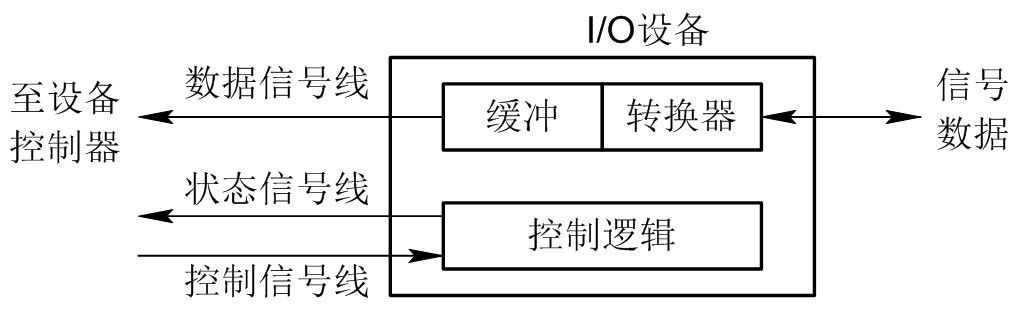
\includegraphics[width=0.9\textwidth]{figure/dev-interface.jpg}
  \end{center}
  \begin{easylist}
    & 数据信号线
    && 在设备与设备控制器之间传送数据信号
    & 状态信号线
    && 传送指示设备当前状态的信号
    & 控制信号线
    && 设备控制器向I/O设备发送控制信号用
  \end{easylist}
\end{frame}

\begin{frame}[fragile]{设备与控制器之间的接口传递的信号}
  \begin{enumerate}
    \item 数据信号:——双向,有缓存
    \item 控制信号:控制器发给设备;要求其完成相关操作
    \item 状态信号:设备发给控制器,后者“显示”;
  \end{enumerate}

  \begin{easylist}
    & IO设备控制的变化
    && 两级(CPU $\leftrightarrow$ IO设备)
    && 三级(CPU $\leftrightarrow$ 控制器  $\leftrightarrow$ IO设备)
    && 四级(CPU $\leftrightarrow$ IO通道 $\leftrightarrow$ 控制器  $\leftrightarrow$ IO设备)
  \end{easylist}
\end{frame}

\begin{frame}[fragile]{讨论:促使IO控制不断发展的推动因素}
  \pause
  \begin{easylist}
    & 减少CPU对IO的干预,充分利用CPU的处理能力
    & 缓和速度不匹配问题
    & 提高CPU和IO的并行程度,使CPU和IO尽可能忙碌。
  \end{easylist}
\end{frame}


\subsubsection{5.1.2 设备控制器}
\begin{frame}[fragile]{5.1.2 设备控制器}
  \begin{easylist}
    & 分类
    && 控制块设备的控制器
    && 控制字符设备的控制器
    & 设备控制器的基本功能
    & 设备控制器的组成
  \end{easylist}
\end{frame}

\begin{frame}[fragile]{设备控制器的基本功能}
  \begin{easylist}
    & 接收CPU命令,控制I/O设备工作,解放CPU.
    & 1.接收和识别命令。
    && 应有相应的Register来存放命令(“命令寄存器”)
    & 2.数据交换:\small{ CPU $\leftrightarrow$ 控制器的数据寄存器  $\leftrightarrow$ 设备}
    & 3.设备状态的了解和报告
    && 设备控制器中的“状态寄存器” 
    & 4.地址识别
    && CPU通过“地址”与设备通信,设备控制器应能识别它所控制的设备地址以及其各寄存
    器的地址。
    & 5.数据缓冲
    && 适配高速的CUP和内存与低速的外设之间的问题
    & 6.差错控制
    && 对由IO设备传来的数据进行差错检测
  \end{easylist}
\end{frame}

\begin{frame}[fragile]{设备控制器组成}
  \begin{easylist}
    & 设备控制器与处理机的接口
    && 实现CPU与控制器通信,共有三类信号线:数据线、地址线和控制线
    && 两类寄存器:数据寄存器、控制/状态寄存器
    & 设备控制器与设备的接口
    && 一个设备控制器连接一个或多个设备,每个接口中都存有数据、控制、状态三种类型的信号
    & I/O逻辑:在其控制下完成与CPU、设备的通信。
  \end{easylist}
\end{frame}

\begin{frame}[fragile]{设备控制器的组成示意图}
  \begin{center}
    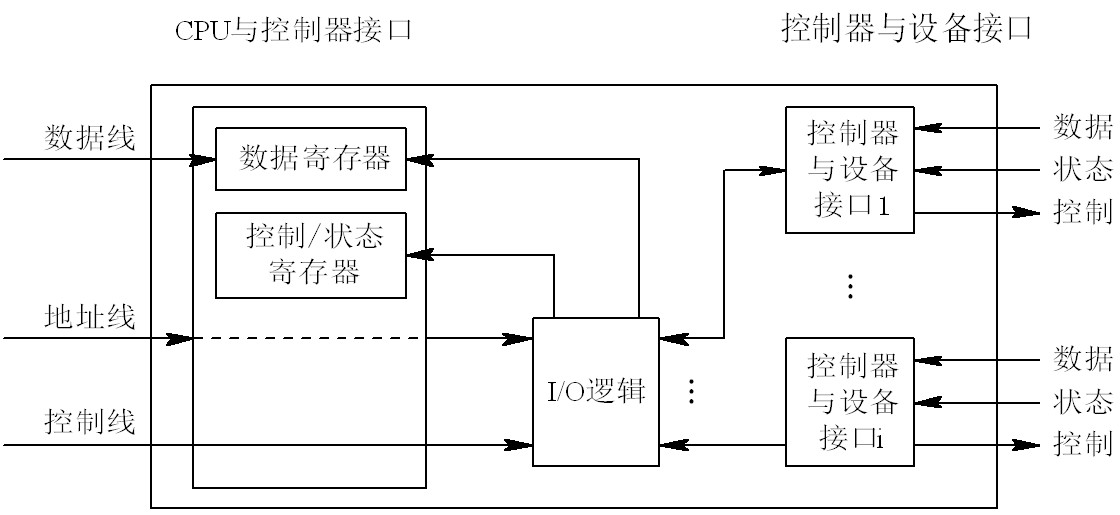
\includegraphics[width=0.9\textwidth]{figure/dev-controller.jpg}
  \end{center}
\end{frame}


\subsubsection{5.1.3 IO通道}
\begin{frame}[fragile]{5.1.3 IO通道}
  \begin{easylist}
    & 通道
    && 一种特殊的执行I/O指令的处理机,与CPU共享内存,可以有自己的总线。
    & 引入目的
    && 解脱CPU对I/O的组织、管理:建立独立的I/O操作,不仅使数据的传送能力独立于
    CPU,而且对有关对I/O操作的组织、管理及其结束处理也尽量独立,以保证CPU有更多
    的时间去进行数据处理。
    & CPU只需发送I/O命令给通道,通道通过调用内存中的相应通道程序完成任务。
    & I/O通道是一种特殊的处理机,具有执行I/O指令的能力,并通过执行通道(I/O)程序
    来控制I/O操作
  \end{easylist}
\end{frame}

\begin{frame}[fragile]{I/O通道与一般的处理机的区别}
  \begin{easylist}
    & 指令类型单一
    & 通道没有自己的内存,通道与CPU共享内存
    & 因为简单,所以价格便宜
  \end{easylist}
\end{frame}

\begin{frame}[fragile]{IO通道的类型}
  \begin{easylist}
    & 1.字节多路通道:
    && 各子通道以时间片轮转方式共享通道,适用于低、中速设备。
    & 2.数组选择通道:
    && 无子通道,仅一主通道,某时间由某设备独占,适于高速设备。
    && 但通道未共享,利用率低。
    & 3.数组多路通道:
    && 多子通道不是以时间片方式,而是“按需分配”,综合了前面2种通道类型的优点。
  \end{easylist}
\end{frame}

\begin{frame}[fragile]{I/O设备通道连接方式 }
  \begin{center}
    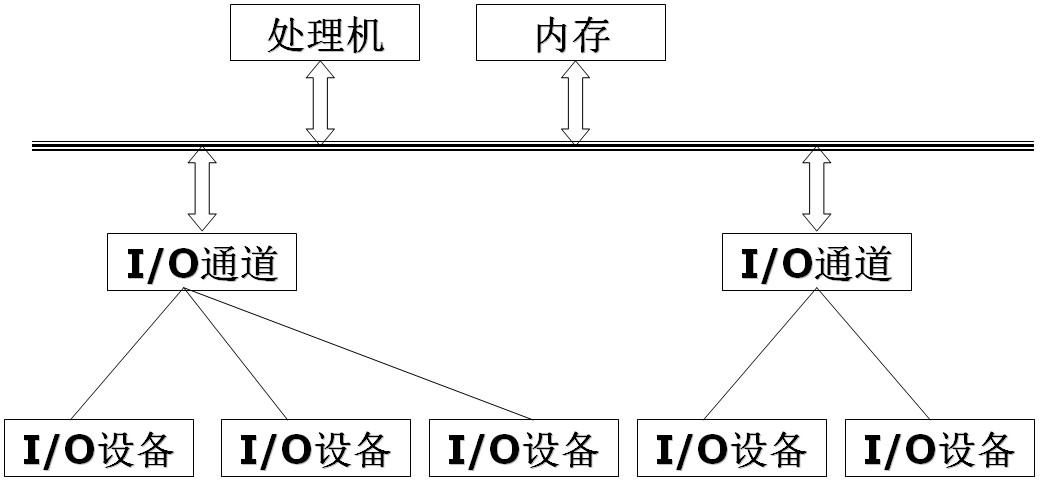
\includegraphics[width=0.9\textwidth]{figure/dev-channel.jpg}
  \end{center}
\end{frame}

\begin{frame}[fragile]{单通路通道“瓶颈”问题}
  \begin{center}
    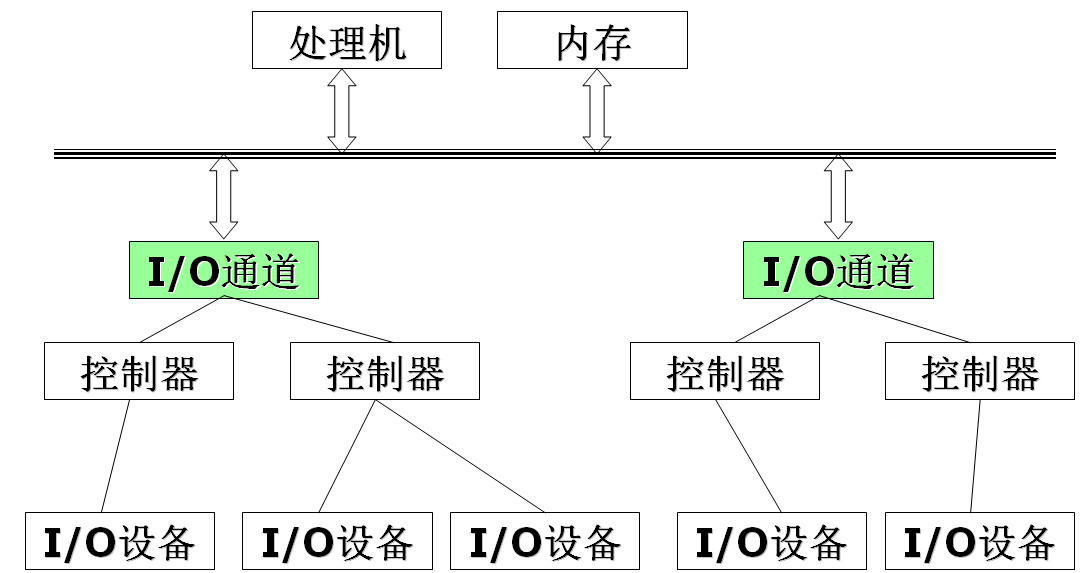
\includegraphics[width=0.9\textwidth]{figure/dev-channel2.jpg}
  \end{center}
\end{frame}

\begin{frame}[fragile]{采用复联方式-多通路}
  \begin{center}
    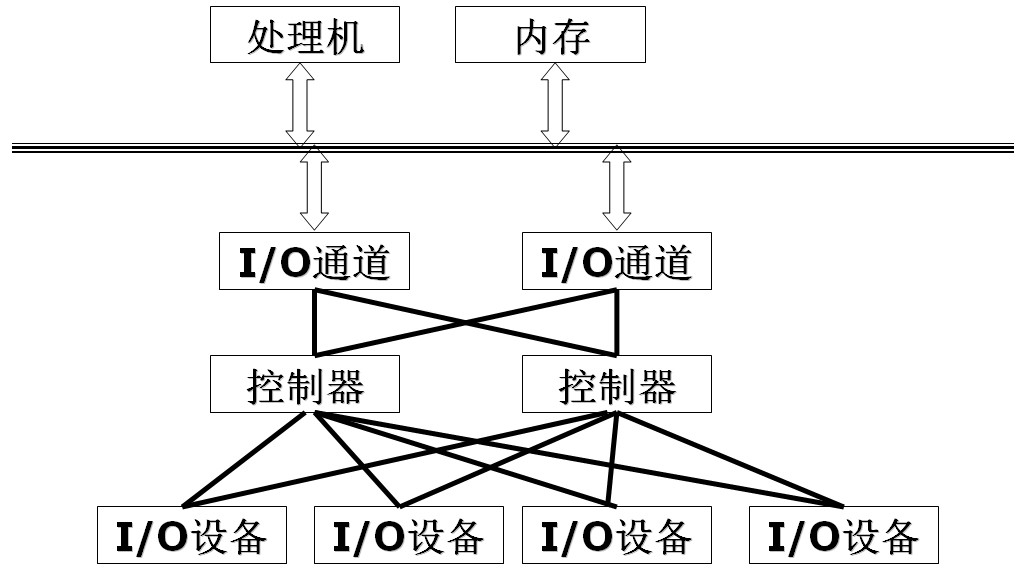
\includegraphics[width=0.9\textwidth]{figure/dev-channel3.jpg}
  \end{center}
\end{frame}

\subsubsection{5.1.4 总线系统}
\begin{frame}[fragile]{5.1.4 总线系统}
  \begin{easylist}
    & 一、微机I/O系统
    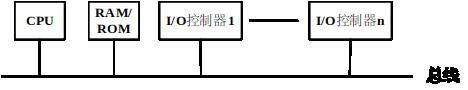
\includegraphics[width=0.8\textwidth]{figure/dev-bus.jpg}

    && 处理机与I/O设备之间的基本连接都是通过总线实现的。即处理机连接在总线上,与
设备无关。设备则根据需要连接在相应的总线上,可多可少,结构和安装均十分灵活
    &&& 如:磁盘设备,打印设备; 缺点:总线瓶颈,CPU瓶颈。
    && ISA/EISA/Local BUS/VESA/PCI 

    & 二、主机I/O系统(四级结构)
    && 计算机—I/O通道—I/O控制器—设备
    && I/O通道相当于对总线的扩展,即多总线方式,且通道有一定的智能性,能与CPU并
行,解决其负担。
    \end{easylist}
\end{frame}


\subsection{5.2 I/O控制方式}
\begin{frame}[fragile]{5.2 I/O控制方式}
  \begin{easylist}
    & 四个发展阶段:
    && 程序I/O
    && 中断I/O
    && DMA控制
    && 通道控制。
    \vspace{1cm}
    & 趋势:提高并行度。
  \end{easylist}
\end{frame}

\subsubsection{5.2.1 程序I/O(忙—等待方式)}
\begin{frame}[fragile]{5.2.1 程序I/O(忙—等待方式)}
  \begin{columns}[onlytextwidth,T]
    \begin{column}{0.45\textwidth}
      \begin{itemize}
        \item 查询方式:CPU需花代价不断查询I/O状态
        \item CPU资源浪费极大。
        \item 例:99.9ms+0.1ms=100ms  
        \item 99.9在忙等
      \end{itemize}
    \end{column}
    \begin{column}{0.55\textwidth}
      \scalebox{0.6}{        
        \begin{tikzpicture}[c/.style={align=center, draw, minimum width=3cm}]
          \small
          \coordinate (top) at (0,0);
          \coordinate (ltop) at (-3,0);
          \draw node[c, below=0.5 of top] (b1) {向I/O控制器\\发读命令} node[right=0.5 of b1] {CPU $\rightarrow$ I/O}
          node[c, below=0.5 of b1] (b2) {读I/O控制器\\的状态}  node[right=0.5 of b2] {I/O $\rightarrow$ CPU}
          node[c, below=0.5 of b2, diamond, inner sep=-0.1cm] (b3) {检查\\状态?} node[right=of b3] (b3r) {出错}
          node[c, below=0.5 of b3] (b4) {从I/O控制器\\中读入字}  node[right=0.5 of b4] {I/O $\rightarrow$ CPU}
          node[c, below=0.5 of b4] (b5) {向存储器\\中写字}  node[right=0.5 of b5] {CPU $\rightarrow$ 内存}
          node[c, below=0.5 of b5, diamond, inner sep=-0.1cm] (b6) {传送\\完成?}
          node[below=0.5 of b6] (b7) {下条指令};

          \coordinate (mtop) at ($(b1)!.45!(b2)$);
          \coordinate (lmtop) at (mtop)[xshift=-2cm];

          \path[->] (b1) edge (b2) (b2) edge (b3) (b3) edge (b4) (b4) edge (b5) (b5) edge (b6) (b6) edge node[right]{完成} (b7) (b3) edge (b3r) (top) ++(0,0.3cm) edge (b1);

          \draw[->] (b3.west) -- ++(-1,0) |- ($(b1)!.45!(b2)$) node[align=center, left=0.5 of b2]{未\\就\\绪};
          \draw[->] (b6.west) -| (ltop) --(top) node[align=center, left=0.1 of b6, yshift=0.3cm]{未完};
        \end{tikzpicture}
      }
    \end{column}
  \end{columns}
\end{frame}


\subsubsection{5.2.2 中断I/O}
\begin{frame}[fragile]{5.2.2 中断I/O}
  \begin{columns}[onlytextwidth,T]
    \begin{column}{0.45\textwidth}
      \begin{itemize}
        \item 向I/O发命令$\rightarrow$返回$\rightarrow$执行其它任务。
        \item I/O中断产生$\rightarrow$CPU转相应中断处理程序。
        \item 如:读数据,读完后以中断方式通知CPU,CPU完成数据从I/O$\rightarrow$内存
        \item 以字(节)为单位进行干预
        \item CPU、设备并行工作
        \item 提高了系统的资源利用率和吞吐量
      \end{itemize}
    \end{column}
    \begin{column}{0.55\textwidth}
      \scalebox{0.6}{        
        \begin{tikzpicture}[c/.style={align=center, draw, minimum width=3cm}]
          \small
          \coordinate (top) at (0,0);
          \coordinate (ltop) at (-3,0);
          \draw node[c, below=0.5 of top] (b1) {向I/O控制器\\发读命令} node[right=0.5 of b1, yshift=0.3cm] {CPU $\rightarrow$ I/O} node[right=0.8 of b1, yshift=-0.3cm] (b1r2) {CPU做其他事情}
          node[c, below=0.5 of b1] (b2) {读I/O控制器\\的状态}  node[right=0.5 of b2,yshift=-0.3cm] {I/O $\rightarrow$ CPU} node[right=0.8 of b2,yshift=0.3cm] (b2r1) {中断} 
          node[c, below=0.5 of b2, diamond, inner sep=-0.1cm] (b3) {检查\\状态?} node[right=of b3] (b3r) {出错}
          node[c, below=0.5 of b3] (b4) {从I/O控制器\\中读入字}  node[right=0.5 of b4] {I/O $\rightarrow$ CPU}
          node[c, below=0.5 of b4] (b5) {向存储器\\中写字}  node[right=0.5 of b5] {CPU $\rightarrow$ 内存}
          node[c, below=0.5 of b5, diamond, inner sep=-0.1cm] (b6) {传送\\完成?}
          node[below=0.5 of b6] (b7) {下条指令};

          \draw[<-, dashed] (b1r2.west)--++(-0.7,0);
          \draw[->, dashed] (b2r1.west)--++(-0.7,0);
          \path[->] (b1) edge (b2) (b2) edge (b3) (b3) edge (b4) (b4) edge (b5) (b5) edge (b6) (b6) edge node[right]{完成} (b7) (b3) edge (b3r) (top) ++(0,0.3cm) edge (b1);

          \draw[->] (b6.west) -| (ltop) --(top) node[align=center, left=0.1 of b6, yshift=0.3cm]{未完};
        \end{tikzpicture}
      }
    \end{column}
  \end{columns}
\end{frame}


\subsubsection{5.2.3 DMA方式——用于块设备中}
\begin{frame}[fragile]{5.2.3 DMA方式——用于块设备中}
  \begin{easylist}
    & 一、DMA(Direct Memory Access)控制方式的引入
    && 中断I/O,CPU按字节干预,即每字节传送产生一次中断。
    && DMA:由DMA控制器直接控制总线传递数据块。DMA控制器完成从I/O——内存。
    & 特点:
    && ① 数据传输的基本单位是数据块,即在CPU与I/O设备之间,每次传送至少一个数据
    块;
    && ② 所传送数据从设备直接送入内存,或者相反;
    && ③ 仅在传送一个或多个数据块的开始和结束时,才需CPU干预,整块数据的传送由控
    制器控制完成。
    & 二、组成
    && 一组寄存器+控制逻辑。
    && CR(命令/状态);  DR(数据);  MAR(内存地址);  DC(计数)
  \end{easylist}
\end{frame}

\begin{frame}[fragile]{DMA控制器的组成图}
  \begin{center}
    \scalebox{0.7}{
      \begin{tikzpicture}[c/.style={align=center, draw, minimum width=1cm, minimum height=0.5cm}]
        \draw node[draw, minimum height=3.2cm, minimum width=2cm] (cpu) {} node[above=0.2 of cpu]{CPU}
        node[draw, minimum height=3.2cm, minimum width=2cm, right=0.5 of cpu] (mem) {} node[above=0.2 of mem]{内存}
        node[draw, minimum height=3.2cm, minimum width=6cm, right=0.5 of mem] (dma) {} node[above=0.2 of dma]{主机--控制器接口~~~控制器与块设备接口};

        \draw node[c, minimum height=1.6cm, minimum width=0.6cm, left=0.2 of mem.east, yshift=0.2cm] (mb){} node[left=0.1 of mb](count){count};
        \draw[] (mb.north)--++(-1,0)  (mb.south)--++(-1,0) ;
        \draw[<-] (mb.north) ++(-0.8,0) --++(0,-0.6);
        \draw[<-] (mb.south) ++(-0.8,0) --++(0,0.6);

        \draw node[c, right=1 of mem, yshift=1cm] (dr) {DR}  node[c, below=0.2 of dr] (mar) {MAR}   node[c, below=0.2 of mar] (dc) {DC}   node[c, below=0.2 of dc] (cr) {CR} 
        node[c, right=0.5 of dr, minimum height=2.6cm, yshift=-1.1cm](io) {I/O\\控\\制\\逻\\辑}
        node[c, right=0.5 of io, minimum height=1cm, minimum width=2cm, yshift=0.8cm] (block1) {} node[c, minimum height=1cm, minimum width=2cm, below=0.5 of block1]{};

        \draw[-latex] (mar.west) -- ($(mb.east) + (0,0.8)$);
        \draw[-latex] (dc.west)--(count.south);
        \draw[] (cpu.south) -- ++(0,-1) -| (mem) (mem.south) ++(0,-1) -| (dma);
        \path[-Latex] (cpu.south) ++(0.5,-0.5) edge node[above] {命令} ++(1.5,0);
        \draw node[below=0.3 of mem, xshift=2cm]{系统总线} node[below=0.2 of dma, xshift=2cm]{DMA控制器};
      \end{tikzpicture}
    }
  \end{center}
  \small
  \begin{easylist}
    && 数据寄存器DR: 用于暂存从设备到内存,或从内存到设备的数据
    && 内存地址寄存器MAR: 在输入时,它存放把数据从设备传送到内存的起始目标地址;
    在输出时,它存放由内存到设备的内存源地址
    && 数据计数器DC:  存放本次CPU要读或写的字(节)数
    && 命令/状态寄存器CR。用于接收从CPU发来的I/O命令或有关控制信息, 或设备的状
    态
  \end{easylist}
\end{frame}

\begin{frame}[fragile]{DMA工作过程}
  \begin{center}
    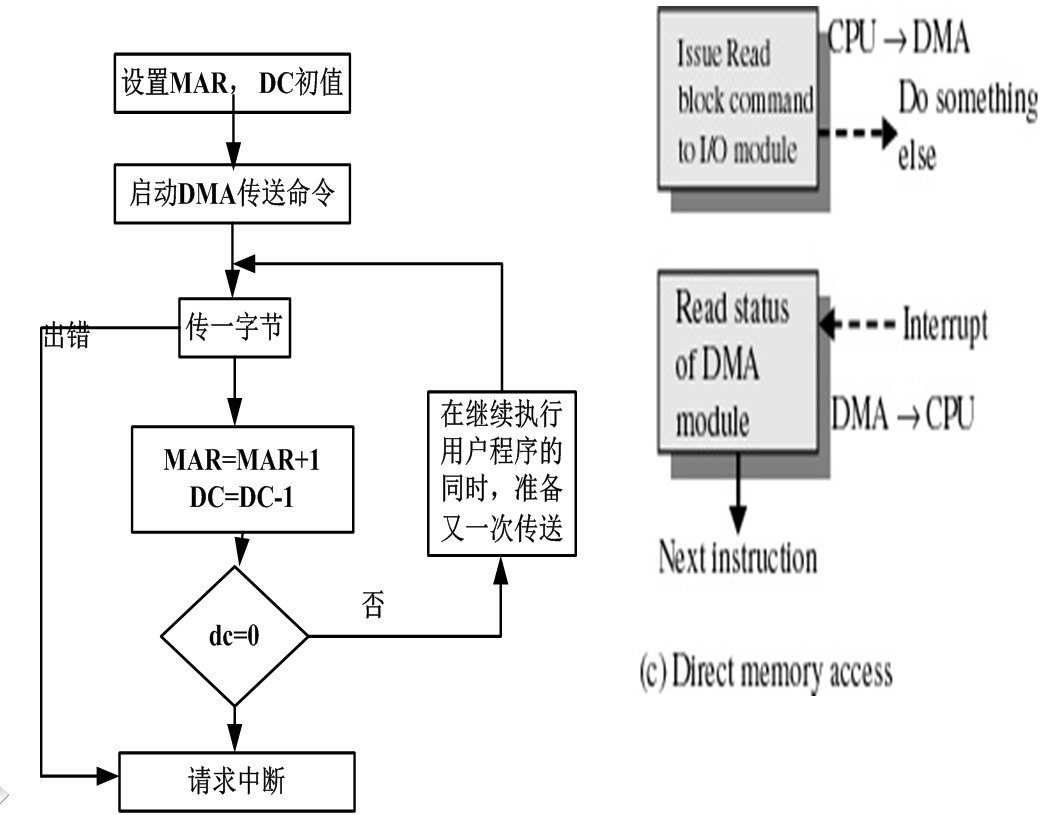
\includegraphics[width=0.75\textwidth]{figure/dev-dma2.jpg}
  \end{center}
\end{frame}

\begin{frame}[fragile]{讨论:中断驱动IO和DMA的区别}
  \begin{easylist}
    & 中断频率
    & 数据的传送方式
  \end{easylist}
\end{frame}

\subsubsection{5.2.4 I/O通道控制方式}
\begin{frame}[fragile]{5.2.4 I/O通道控制方式(1)}
  \begin{easylist}
    & I/O通道控制方式的引入
    && DMA方式:对许多离散块的读取仍需要多次中断。
    && 对一组数据块的读(或写)及有关的控制和管理为单位的干预
    && 实现CPU、通道和I/O设备三者的并行操作,从而更有效地提高整个系统的资源利用率
  \end{easylist}
\end{frame}

\begin{frame}[fragile]{5-2-4  I/O通道控制方式(2)}
  \begin{easylist}
    & 通道方式:CPU只需给出
    && (1)通道程序首址。
    && (2)要访问I/O设备后,通道程序就可完成一组块操作 
  \end{easylist}
\end{frame}

\begin{frame}[fragile]{通道程序的指令信息}
  \begin{easylist}
    & (1)操作码:指令所执行的操作
    & (2)内存地址:字符送入内存(读操作)或从内存取出(写操作)时的内存首址
    & (3)计数:要读写的字节数
    & (4)通道程序结束位P:P=1表示最后一条指令
    & (5)记录结束标志R,R=0,表示本指令和下一条指令处理的数据同属于一个记录。
  \end{easylist}
\end{frame}

\begin{frame}[fragile]{通道程序}
  \begin{easylist}
    & (1) 操作码	(2) 内存地址
    & (3) 计数 	(4) 通道程序结束位P 
    & (5) 记录结束标志R 
  \end{easylist}
  \begin{center}
    \begin{tabular}{|c|c|c|c|c|}
      \hline
      操作 & P & R & 计数 & 内存地址 \\ \hline
      WRITE & 0 & 0 & 80 & 813 \\ \hline
      WRITE & 0 & 0 & 140 & 1034 \\ \hline
      WRITE & 0 & 1 & 60 & 5830 \\ \hline
      WRITE & 0 & 1 & 300 & 2000 \\ \hline
      WRITE & 0 & 0 & 250 & 1850 \\ \hline
      WRITE & 1 & 1 & 250 & 720 \\ \hline
    \end{tabular}
  \end{center}
\end{frame}


\subsection{5.3 缓冲管理}
\begin{frame}[fragile]{5.3 缓冲管理}
~
\end{frame}

\subsubsection{5.3.1 缓冲的引入}
\begin{frame}[fragile]{5.3.1 缓冲的引入}
  \begin{easylist}
    & 1.缓和CPU和I/O设备间速度不匹配的矛盾。
    && 如:计算——打印buffer——打印
    & 2.减少对CPU的中断频率
    && 如:buffer越大,“buffer满”信号发生频率越低。
    & 3.提高CPU和I/O并行性 
  \end{easylist}
\end{frame}

\begin{frame}[fragile]{例子}
  \begin{center}
    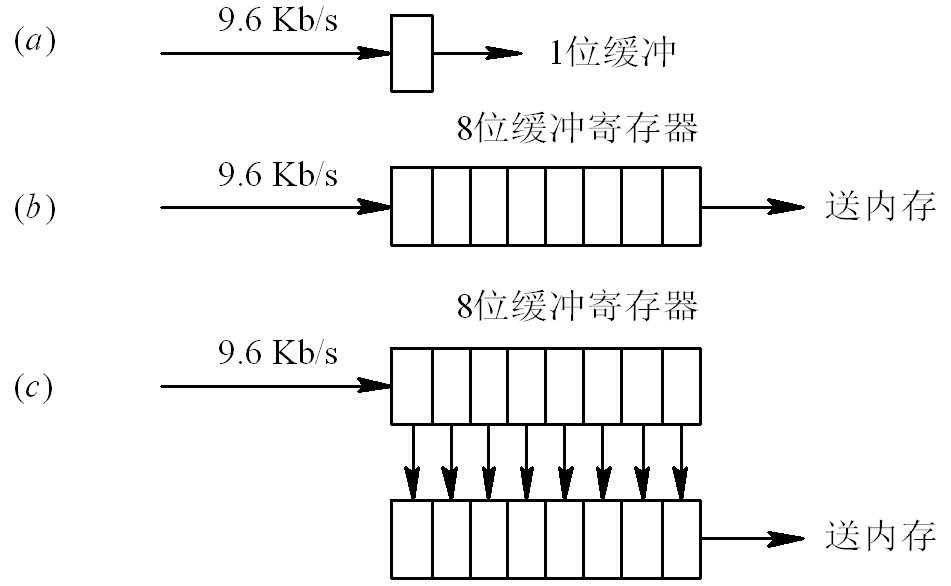
\includegraphics[width=0.7\textwidth]{figure/dev-buffer-demo.jpg}
  \end{center}
  \begin{easylist}
    & (a) CPU中断频率:9.6Kb/s; CPU响应时间:约100us
    & (b) CPU中断频率:1.2Kb/s; CPU响应时间:约800us
    & (c) CPU中断频率:0.6Kb/s; CPU响应时间:约1600us
  \end{easylist}
\end{frame}

\subsubsection{5.3.2 单缓冲和双缓冲}
\begin{frame}[fragile]{5.3.2 单缓冲和双缓冲(1)}
  \begin{easylist}
    & 单缓冲(Single Buffer)
    & 系统对数据的处理时间:Max(C,T)+M
  \end{easylist}
  \begin{center}
    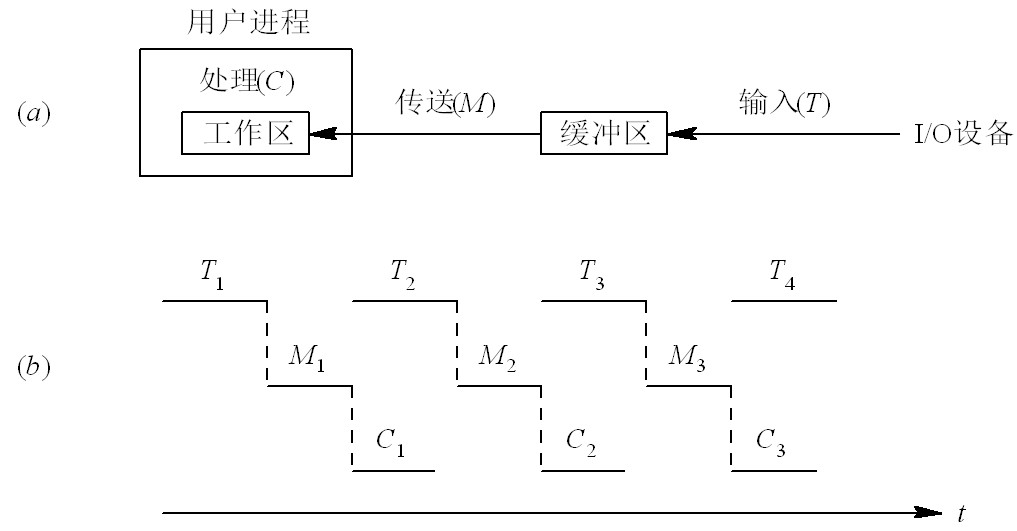
\includegraphics[width=0.9\textwidth]{figure/dev-buffer-single.jpg}
  \end{center}
\end{frame}

\begin{frame}[fragile]{5.3.2 单缓冲和双缓冲(2)}
  \begin{easylist}
    & 双缓冲(Double Buffer)
    & 系统对数据的处理时间:$Max(C+M,T) \approx Max(C, T)$
  \end{easylist}
  \begin{center}
    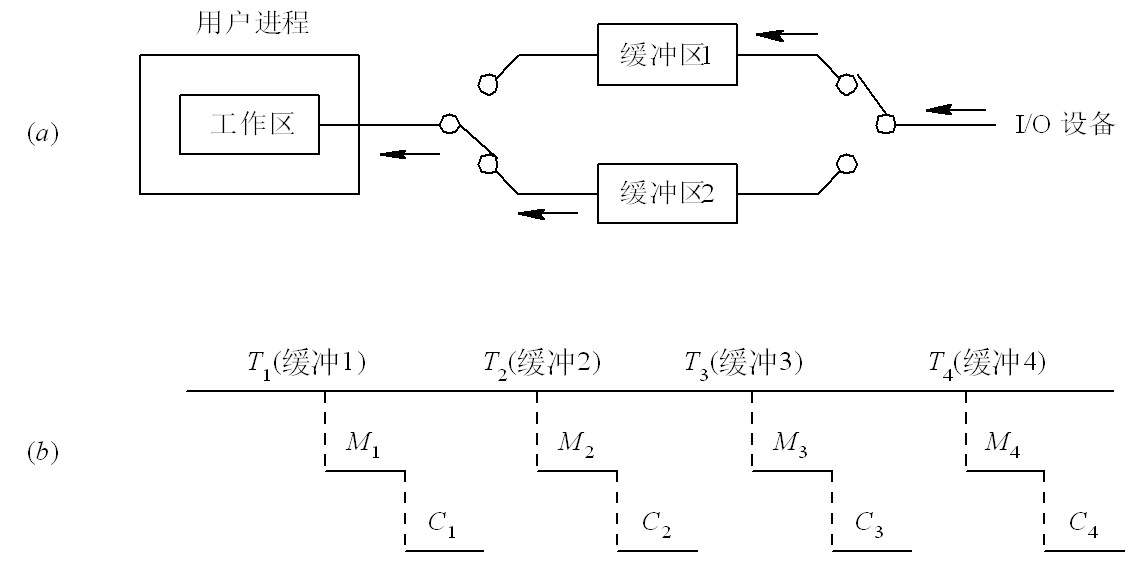
\includegraphics[width=0.8\textwidth]{figure/dev-buffer-double.jpg}
  \end{center}
\end{frame}

\begin{frame}[fragile]{5.3.2 单缓冲和双缓冲(3)}
  \begin{easylist}
    & 双机通信时缓冲区的设置
  \end{easylist}
  \begin{center}
    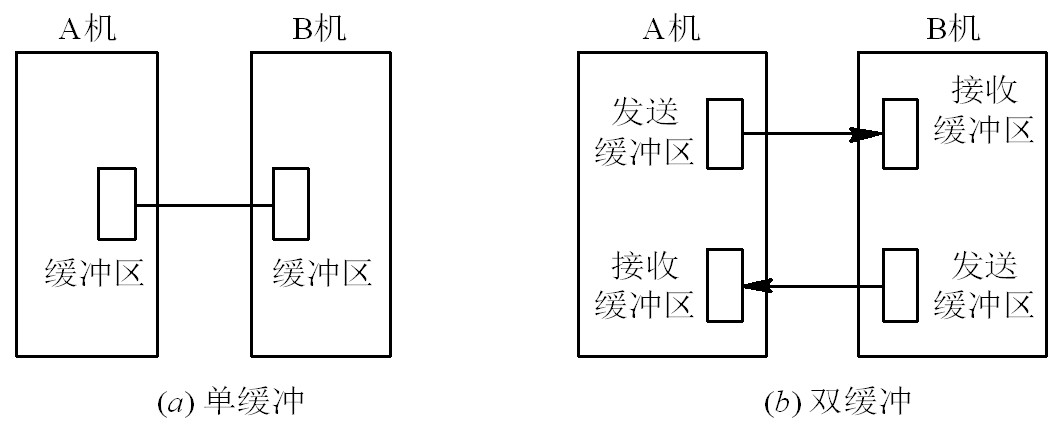
\includegraphics[width=0.9\textwidth]{figure/dev-buffer-two.jpg}
  \end{center}
\end{frame}

\subsubsection{5.3.3 循环缓冲}
\begin{frame}[fragile]{5.3.3 循环缓冲}
  \begin{easylist}
    & 1.循环缓冲的组成 
    && (1)多个缓冲区,三种类型
    &&& 用于装输入数据的空缓冲区R
    &&& 已装满数据的缓冲区G
    &&& 计算进程正在使用的现行工作缓冲区C
    && (2)多个指针
    &&& 指示计算进程下一个可用缓冲区G的指针NextG
    &&& 指示输入进程下次可用的空缓冲区R的指针Nexti
    &&& 指示计算进程正在使用的缓冲区C的指针Current
  \end{easylist}
\end{frame}

\begin{frame}[fragile]{循环缓冲组成示意图}
  \begin{center}
    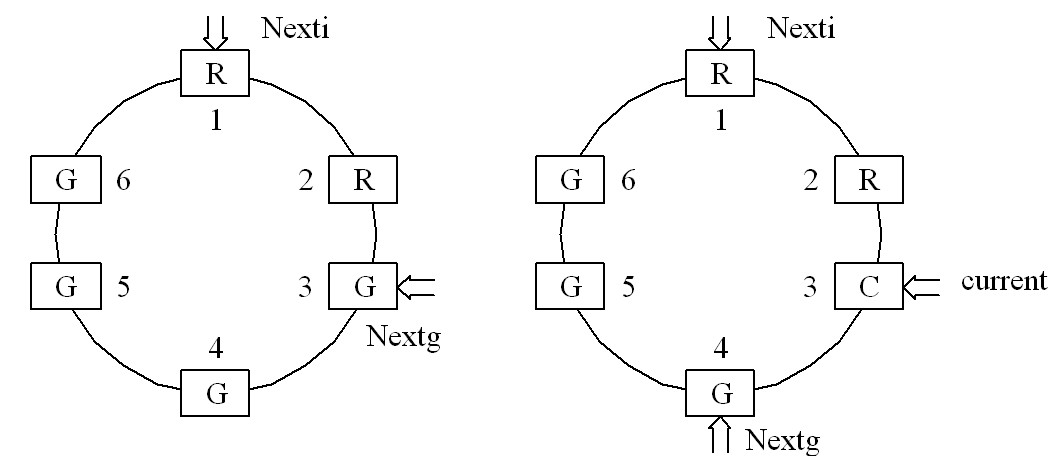
\includegraphics[width=0.8\textwidth]{figure/dev-buffer-loop.jpg}
  \end{center}
  \small
  \begin{easylist}
    & R: 空缓冲区; G: 已装满数据的缓冲区
    & C: 正在使用的现行工作缓冲区
    & Nextg: 指示计算进程下次可用的数据缓冲区的指针
    & Nexti: 指示输入进程下次可用的空缓冲区的指针
    & current: 指示计算进程正在使用的数据缓冲区的指针
  \end{easylist}
\end{frame}

\begin{frame}[fragile]{循环多缓冲的使用}
  \begin{easylist}
    & nextg:指示下一个计算进程应取数据的buf
    & nexti:指示下一个空buf供输入进程使用.
    & Getbuf:
    && 计算进程:取nextg对应缓冲区提供使用,将Nextg置为空,Nextg=(Nextg+1)Mod N
    && 输入进程:将Nexti对应缓冲区提供使用,将Nexti置为满,Nexti=(Nexti+1)Mod N
    & Releasebuf:
    && 输入进程:当把缓冲区C装满后,则改为G缓冲区;
    && 计算进程:当把缓冲区C中的数据提取完毕后,则把C改为R;
  \end{easylist}
\end{frame}

\begin{frame}[fragile]{循环多缓冲的同步问题}
  \begin{easylist}
    & Nexti 追上Nextg:
    && 表示输入速度>输出速度,全部buf满,这时输入进程阻塞,系统受计算能力限制。
    & Nextg追上Nexti:
    && 输入速度<输出速度,全部buf空,这时输出进程阻塞。系统受I/O能力限制。 
  \end{easylist}
\end{frame}

\subsubsection{5.3.4  缓冲池}
\begin{frame}[fragile]{5.3.4  缓冲池}
  \begin{easylist}
    & 缓冲池:系统提供的公用缓冲 
    && 前面的缓冲区仅适用于特定的IO进程和计算进程,属于专用缓冲。
    && 提供可供进程共享的公用缓冲,提高缓冲区利用率
  \end{easylist}
\end{frame}

\begin{frame}[fragile]{1. 缓冲池的组成}
  \begin{easylist}
    & 一、组成:
    && 3个队列:
    &&& 空缓冲队列emq
    &&& 输入队列inq
    &&& 输出队列outq
    && 四个工作缓冲区:
    &&& hin:收容输入数据
    &&& sin:提取输入数据
    &&& hout:收容输出数据
    &&& sout:提取输出数据
  \end{easylist}
\end{frame}

\begin{frame}[fragile]{2. 缓冲池的4种工作方式}
  \begin{easylist}
    & 1.收容输入;
    & 2.提取输入
    & 3.收容输出;
    & 4.提取输出
  \end{easylist}
  \begin{center}
    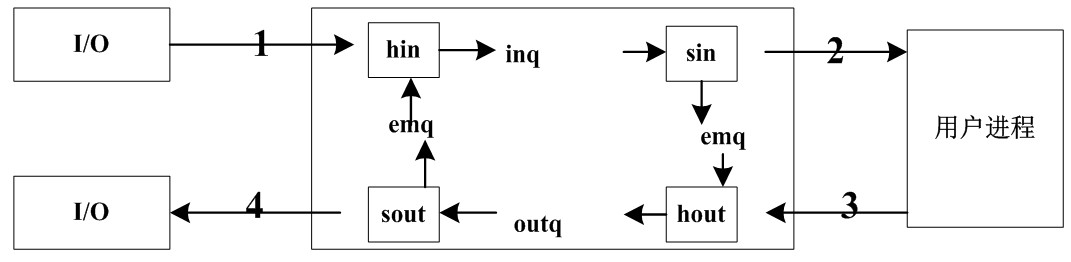
\includegraphics[width=0.9\textwidth]{figure/dev-buffer-pool.jpg}
  \end{center}
\end{frame}

\begin{frame}[fragile]{工作方式}
  \begin{easylist}
    & 1. hin=getbuf(emq);\\
    ~~~ putbuf(inq,hin)
    & 2. sin=getbuf(inq);	\\
    ~~~计算;\\
    ~~~putbuf(emq,sin)
    & 3. hout=getbuf(emq);\\
    ~~~putbuf(outq, hout);
    & 4. sout=getbuf(outq); \\
    ~~~输出;\\
    ~~~putbuf(emq,sout)
  \end{easylist}
\end{frame}

\begin{frame}[fragile]{3. Getbuf和Putbuf过程}
  \begin{columns}[onlytextwidth,T]
    \begin{column}{0.5\textwidth}
      \begin{lstlisting}[tabsize=8,keywordstyle=\color{red},basicstyle=\small,
        language=Pascal, numbers=none]
Getbuf(type)
Begin
  wait(RS(type));
  wait(MS(type));
  B(number):=takebuf(type);
  signal(MS(type));
end
      \end{lstlisting}
    \end{column}      
    \begin{column}{0.5\textwidth}
      \begin{lstlisting}[tabsize=8,keywordstyle=\color{red},basicstyle=\small,
        language=Pascal, numbers=none]
Putbuf(type)
Begin
  wait(MS(type));
  addbuf(type,number);
  signal(MS(type));
  signal(RS(type));
end
      \end{lstlisting}
    \end{column}
  \end{columns}
  \begin{easylist}
    & MS(type)为type类型队列的互斥信号量,保证队列的互斥访问
    & RS(type)为type类型队列的资源信号量,记录资源数量
  \end{easylist}
\end{frame}

\begin{frame}[fragile]{~}
  \begin{easylist}

  \end{easylist}
\end{frame}

\subsection{5.4  设备分配}
\begin{frame}[fragile]{5.4  设备分配}
  \begin{easylist}
    & 多道程序环境下,设备供所有进程共享,为防止进程对系统资源的无序竞争,规定系统设备只能由系统统一分配。设备分配程序按照一定的策略,把设备分配给请求用户。
    & 包括:对设备、设备控制器、通道的分配
  \end{easylist}
\end{frame}


\subsubsection{5.4.1 设备分配的数据结构}
\begin{frame}[fragile]{5.4.1 设备分配的数据结构}
  \begin{easylist}
    & 一、设备控制表DCT:
    && 每个设备一张,记录本设备的情况
    & 二、控制器控制表(COCT),通道表(CHCT),系统设备表(SDT)
    && SDT:记录了系统中全部设备及其驱动程序地址等信息。
  \end{easylist}
\end{frame}

\begin{frame}[fragile]{设备控制表DCT}
  \begin{center}
    \begin{tikzpicture}[c/.style={draw, minimum height=1cm, minimum width=2.5cm},c2/.style={draw, minimum height=0.6cm, minimum width=5.5cm, align=left, text justified=left}]
      \draw[] node[c] (dct1) {$DCT_1$}
      node[c, below=0 of dct1, minimum height=1cm] (dct2) {$\vdots$} 
      node[c, below=0 of dct2] (dct2) {$DCT_i$} 
      node[c, below=0 of dct2, minimum height=1cm] (dcti) {$\vdots$}  node[c, below=0 of dcti] (dctn) {$DCT_n$} 
      node[left=0.5 of dcti, rotate=90, xshift=2cm]{设备控制表集合};

      \draw[] node[c2, right=2 of dct1, yshift=-0.5cm] (t1) {设备类型type~~~~~~~~~~~}
      node[c2, below=0 of t1] (t2) {设备标识符:device\_id}
      node[c2, below=0 of t2] (t3) {设备状态:等待/不等待, 忙/闲}
      node[c2, below=0 of t3, fill=red!10] (t4) {指向控制器表的指针}
      node[c2, below=0 of t4, fill=red!10] (t5) {重复执行次数或时间}
      node[c2, below=0 of t5, fill=red!10] (t6) {设备队列的队首指针};

      \draw[-Latex, dashed, thick] (dct2.east) ++(0,0.5) -- ($(t1.west) + (0,0.3)$);
      \draw[-Latex, dashed, thick] (dct2.east) ++(0,-0.5) -- ($(t6.west) + (0,-0.3)$);
    \end{tikzpicture} 
  \end{center}
  \begin{easylist}
    & 一个设备一张设备控制表,记录本设备的情况
  \end{easylist}
\end{frame}

\begin{frame}[fragile]{控制器控制表}
  \begin{easylist}
    & 一个控制器一个COCT表,记录本控制器情况
  \end{easylist}
  \begin{center}
    \begin{tikzpicture}[c/.style={draw, minimum height=1cm, minimum width=5cm}]
      \draw[] node[c] (t1) {控制器标识符:controller\_id}
      node[c, below=0 of t1] (t2) {控制器状态:忙/闲}
      node[c, below=0 of t2] (t3) {与控制器连接的通道表指针}
      node[c, below=0 of t3] (t4) {控制器队列的队首指针}
      node[c, below=0 of t4] (t5) {控制器队列的队尾指针}
      node[below=0.5 of t5] {控制器表COCT};
    \end{tikzpicture} 
  \end{center}
\end{frame}

\begin{frame}[fragile]{通道控制表}
  \begin{easylist}
    & 一个通道一张通道控制表
  \end{easylist}
  \begin{center}
    \begin{tikzpicture}[c/.style={draw, minimum height=1cm, minimum width=5cm}]
      \draw[] node[c] (t1) {通道标识符:channel\_id}
      node[c, below=0 of t1] (t2) {通道状态:忙/闲}
      node[c, below=0 of t2] (t3) {与通道连接的控制器表指针}
      node[c, below=0 of t3] (t4) {通道队列的队首指针}
      node[c, below=0 of t4] (t5) {通道队列的队尾指针}
      node[below=0.5 of t5] {通道表CHCT};
    \end{tikzpicture} 
  \end{center}
\end{frame}

\begin{frame}[fragile]{系统设备表}
  \begin{easylist}
    & 记录系统中全部设备的情况
  \end{easylist}
  \begin{center}
    \begin{tikzpicture}[c/.style={draw, minimum height=1cm, minimum width=2.5cm},c2/.style={draw, minimum height=0.8cm, minimum width=4cm, align=left, text justified=left}]
      \draw[] node[c] (dct1) {表目1}
      node[c, below=0 of dct1, minimum height=1cm] (dct2) {$\vdots$} 
      node[c, below=0 of dct2] (dct2) {表目i} 
      node[c, below=0 of dct2, minimum height=1cm] (dcti) {$\vdots$}
      node[below=0.5 of dcti, xshift=3cm]{系统设备表SDT} ;

      \draw[] node[c2, right=2 of dct1] (t1) {设备类}
      node[c2, below=0 of t1] (t2) {设备标识符}
      node[c2, below=0 of t2] (t3) {DCT}
      node[c2, below=0 of t3, fill=red!10] (t4) {驱动程序入口};

      \draw[-Latex, dashed, thick] (dct2.east) ++(0,0.5) -- ($(t1.west) + (0,0.3)$);
      \draw[-Latex, dashed, thick] (dct2.east) ++(0,-0.5) -- ($(t4.west) + (0,-0.3)$);
    \end{tikzpicture} 
  \end{center}
\end{frame}

\subsubsection{5.4.2 设备分配应考虑的若干因素}
\begin{frame}[fragile, allowframebreaks]{5.4.2 设备分配应考虑的若干因素}
  \begin{easylist}
    & 一、设备的固有属性:
    && (1) 独享设备:采用独享分配策略 
    && (2) 共享设备:注意调度 
    && (3) 虚拟设备
    & 二、分配算法:
    && (1) FIFO;
    && (2) 优先权。
    & 三、安全性:
    && 方式1:安全分配(同步):每进程获得一I/O后,即block,直到其I/O完成。
    &&& 即打破了死锁条件。
    &&& 缺点:CPU、I/O对该进程是串行,进程进展缓慢。
    && 方式2:不安全分配(异步):进程在发出IO请求后仍继续运行,可继续请求第二个
    IO需求;
    &&& 需进行安全性检查,进程执行效率高。
    & 四、设备独立性
    && 5.4.3内容
  \end{easylist}
\end{frame}

\subsubsection{5.4.3 设备独立性}
\begin{frame}[fragile]{5.4.3 设备独立性}
  \begin{easylist}
    & 1、设备独立性概念
    && 即设备无关性,指应用程序独立于具体使用的物理设备。
    &&& 例:打印时的打印机选择
    && 为实现设备独立性引入逻辑设备和物理设备概念
    &&& 在应用程序中,使用逻辑设备名称来请求使用某类设备;而系统在实际执行时,还
    必须使用物理设备名称。因此,系统须具有将逻辑设备名称转换为某物理设备名称的功
    能,类似于存储器管理中的逻辑地址与物理地址关系。
    && 逻辑设备表(LUT:Logical Unit Table):
  \end{easylist}
  \begin{center}
    \begin{tikzpicture}[c/.style={draw, minimum height=1cm, minimum width=2.5cm}]
      \draw[] node[c] (b1) {逻辑设备} node[c, right=0 of b1] (b2) {物理设备} node[c, right=0 of b2]{Driver入口};
    \end{tikzpicture} 
  \end{center}
\end{frame}

\begin{frame}[fragile]{1、设备独立性的概念-续}
  \begin{easylist}
    & 分配流程:进程给出逻辑名$\rightarrow$通过LUT得到物理设备及其driver入口。
    & 优点:
    && 设备分配更灵活;
    &&& 逻辑设备和物理设备间可以是多---多的映射关系。提高了物理设备的共享性,以及使用的灵活性。如:
    &&&& 某逻辑名可对应这一类设备,提高均衡性与容错性。
    &&&& 几个逻辑名可对应某一个设备,提高共享性。
    && 易于实现I/O重定向。
    &&& 不变程序,只需改变LUT表的映射关系。
    &&& 如调式时输出到屏幕,测试成功后输出到打印机
  \end{easylist}
\end{frame}

\begin{frame}[fragile]{2、设备独立性软件}
  \begin{easylist}
    & 执行所有设备的公有操作
    && 分配回收:对独立设备的分配与回收
    && 名字映射:将逻辑设备名映射为物理设备名,进一步可以找到相应物理设备的驱动程序
    && 保护:对设备进行保护,禁止用户直接访问设备
    && 缓冲管理:即对字符设备和块设备的缓冲区进行有效的管理, 以提高I/O的效率;
    && 差错控制:处理设备驱动程序无法处理的错误
    & 向用户层软件提供统一接口
    && 无论何种设备, 它们向用户所提供的接口应该是相同的,如统一的Read和Write操作
  \end{easylist}
\end{frame}

\begin{frame}[fragile]{例}
  \begin{lstlisting}[tabsize=8,keywordstyle=\color{red},basicstyle=\small,
    language=Pascal, numbers=none]
struct general_op{
    int (*read)(…)
    int (*write)(…)
};

driver1: struct  general_op dev_op={  
    dev1_read,
    dev1_write
};
driver2: struct  general_op dev_op={  
    dev2_read,
    dev2_write
};
Gen_read(fd,…){
    dev_op=map(fd);
    dev_op->read(…);
}
  \end{lstlisting}
\end{frame}

\begin{frame}[fragile]{3、逻辑设备名到物理设备名映射的实现}
  \begin{easylist}
    & 1) 逻辑设备表:用于将应用程序中所使用的逻辑设备名映射为物理设备名
    & 2) LUT的设置问题:
    && (a) 系统中只设置一张LUT: 所有用户之间不允许有相关的逻辑设备名
    && (b) 一个用户一张LUT: 多用户系统中通常都配置系统设备表,故只需给出系统设备
    表的指针即可
  \end{easylist}

  \small
  \begin{columns}[onlytextwidth,T]
    \begin{column}{0.45\textwidth}
      \begin{tabular}{|c|c|c|}
        \hline
        \rowcolor{green!10}
        逻辑设备名 & 物理设备名 & \tabincell{c}{驱动程序\\入口地址} \\ \hline
        /dev/tty & 3 & 1024 \\ \hline
        /dev/printer & 5 & 2046 \\ \hline
        $\cdots$ & $\cdots$ & $\cdots$ \\ \hline
      \end{tabular}
      \begin{center}
        (a)
      \end{center}
    \end{column} 

    \begin{column}{0.45\textwidth}
      \begin{tabular}{|c|c|}
        \hline
        \rowcolor{green!10}
        逻辑设备名 & \tabincell{c}{系统设备\\表指针} \\ \hline
        /dev/tty & 3 \\ \hline
        /dev/printer & 5 \\ \hline
        $\cdots$ & $\cdots$ \\ \hline
      \end{tabular}
      \begin{center}
        (b)
      \end{center}
    \end{column}
  \end{columns}
\end{frame}

\subsubsection{5.4.4 独占设备的分配程序}
\begin{frame}[fragile, allowframebreaks]{5.4.4 独占设备的分配程序}
  \begin{easylist}
    & 1. 基本的设备分配程序 
    && 1)分配设备 
    && 2)分配控制器 
    && 3)分配通道 
    && 只有在设备、控制器和通道三者都分配成功时,此次设备分配才算成功
    \newpage
    & 2. 设备分配程序的改进
    && 1)增加设备的独立性:使用逻辑设备名请求I/O 
    &&& 系统首先从SDT中找出第一个该类设备的DCT,如忙,则找下一个,仅当所有该类设
    备都忙时,才把进程挂在该类设备的等待队列上。
    && 2)考虑多通路情况 
    &&& 设备(控制器)所连接的第一个控制器(通道)忙时,则查看所连接的第二个控制
    器(通道),只有都忙时,才把进程挂在控制器(通道)的等待队列上
  \end{easylist}
\end{frame}

\begin{frame}[fragile, allowframebreaks]{分配程序示例}
  \begin{easylist}
    & 进程n请求设备:
  \end{easylist}

  \begin{lstlisting}[tabsize=8,keywordstyle=\color{red},basicstyle=\small,
    language=Pascal]
  search (sdt, phdevice);

  if not busy (phdevice) then
    begin
      compute(safe); //对独占设备
      if safe then
         alloc (n, phdevice);
      else begin
         insert (DL(phdevice), n); //将n插入设备等待队列DL上
         return;
      end;
    end;
  else begin //设备忙
      insert (DL (phdevice), n);
      return;	
  end;

  //device分配成功
  
  controllerid=controllerid (COCT ptr(dct)); 
  if not busy (COCT (controllerid)) then
      alloc (n, controllerid); 
  else begin
     insert (col, n);
     return;
  end;

  //控制器分配成功

  channeled=channeled(chatptr (controllerid)); 
  if not busy (chct (channelid)) then
      allocation (n, channelid);
  else begin
     insert (chl, n)
     return;
   end;
  \end{lstlisting}  

  \begin{easylist}
    & 优化:
    && 1)增加设备的独立性
    && 2)考虑多通路情况
  \end{easylist}
\end{frame}


\subsubsection{5.4.5 SPOOLing技术 }
\begin{frame}[fragile]{5.4.5 SPOOLing技术 }
  虚拟性:单一物理CPU被虚拟成多台逻辑CPU,同样可以想法把单一物理设备虚拟为多台逻
  辑设备

  \begin{easylist}
    & 1. SPOOLling的基本概念
    & 2. SPOOLing组成
    & 3. 共享打印机
    & 4. SPOOLing的特点
  \end{easylist}
\end{frame}

\begin{frame}[fragile]{1. SPOOLing的基本概念}
  \begin{easylist}
    & 把在联机情况下实现的同时外围操作称为SPOOLing (Simultaneaus Periphernal
    Operating On-Line),或称为假脱机操作。
    & 作用:
    && 通过缓冲方式,将独占设备改造为共享设备 
  \end{easylist}
\end{frame}

\begin{frame}[fragile]{2. SPOOLing组成}
  \begin{easylist}
    & 1.输入井和输出井:
    && 在磁盘上开辟的2个大存储空间,模拟输入和输出设备。
    & 2.输入buf和输出buf(内存中)
    && (1) 输入设备 $\rightarrow$ 输入buf $\rightarrow$ 输入井 $\rightarrow$ 用户区
    && (2) 用户区 $\rightarrow$ 输出井 $\rightarrow$ 输出buf $\rightarrow$ 设备
    & 3.输入$SP_i$和输出$SP_o$进程。
    && 分别控制(1), (2)的动作。
    && $SP_i$相当于脱机输入控制器。
    && $SP_o$相当于脱机输出控制器。
  \end{easylist}
\end{frame}

\begin{frame}[fragile]{SPOOLing系统的组成示意图}
  \begin{center}
    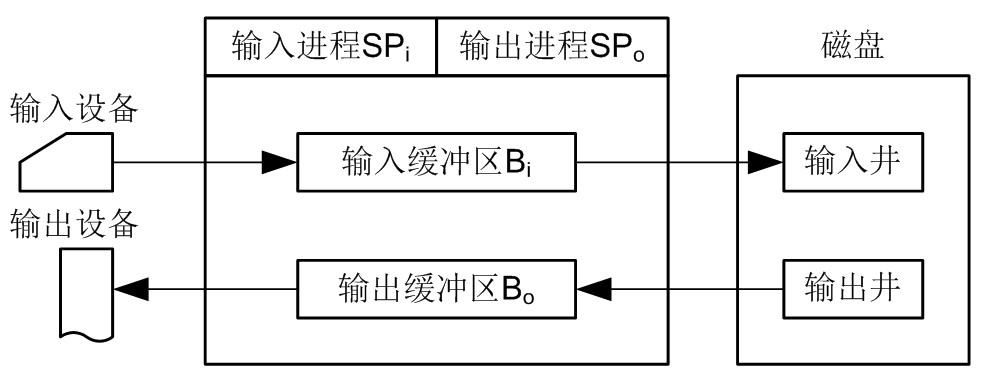
\includegraphics[width=0.9\textwidth]{figure/dev-spooling.jpg}
  \end{center}
\end{frame}

\begin{frame}[fragile]{3. 共享打印机}
  \begin{easylist}
    & 共享打印机技术已被广泛地用于多用户系统和局域网络中。当用户进程请求打印输出
    时,SPOOLing系统同意为它打印输出, 但并不真正立即把打印机分配给该用户进程,
    而只为它做两件事: 
    && (1) 由输出进程在输出井中为之申请一个空闲磁盘块区,并将要打印的数据送入其
    中
    && (2) 输出进程再为用户进程申请一张空白的用户请求打印表,并将用户的打印要求
    填入其中, 再将该表挂到请求打印队列上
  \end{easylist}
\end{frame}

% \begin{frame}[fragile]{共享打印机过程}
%   \begin{easylist}
%     & (1)输入
%     && a. 进程n请求 $\rightarrow$ SPi为n在输入井中分配空间 $\rightarrow$ 设备数
%     据由输入buf送输入井 $\rightarrow$ 生成输入请求表挂输入请求队列。
%     && b. CPU空闲 $\rightarrow$ 取请求表中的任务,送进程缓冲区。
%     & (2)输出:(打印)
%     && a. 进程n请求 $\rightarrow$ SPo为n在输出井中分配空间 $\rightarrow$ 将数据
%     由进程buf转到输出井 $\rightarrow$ 生成一打印请求表挂打印请求队列。
%     && b. 打印机空 $\rightarrow$ 查打印请求表中的任务 $\rightarrow$ 取输出井中对
%     应数据 $\rightarrow$ 输出buf $\rightarrow$ 打印
%   \end{easylist}
% \end{frame}

\begin{frame}[fragile]{4. SPOOLing的特点 }
  \begin{easylist}
    & 1.提高I/O速度:
    && 对低速设备操作 $\rightarrow$ 变为对输入/输出井操作。
    & 2.将独占设备改造为共享设备
    && 分配设备的实质是分配输入/出井
    & 3.实现了虚拟设备功能
    && 对于独占设备,用户都感到是自己独占了该设备。
  \end{easylist}
\end{frame}

\begin{frame}[fragile]{讨论:SPOOLing和缓冲的区别}
  \pause
  \begin{easylist}
    & 目的不同:
    && SPOOLing解决的是独占I/O设备如何共享使用的问题
    && 缓冲解决的是I/O设备和CPU的速度不匹配的问题。
    & 数据存放的位置
    && SPOOLing在磁盘上开辟输入井和输出井
    && 缓冲在内存中设置缓冲区
    & 管理
    && SPOOLing由井管理程序负责
    && 缓冲由缓冲区管理软件负责
  \end{easylist}
\end{frame}



\subsection{5.5 设备处理}
\begin{frame}[fragile]{5.5 设备处理}
  \begin{easylist}
    & 设备处理程序即是设备驱动程序
    && 设备处理程序用于实现I/O进程与设备控制器之间的通信,由于常以进程形式存在,
    故可简称为设备驱动进程
    && 负责接收上层软件发来的抽象要求,再转换为具体要求后,发送给设备控制器,启
    动设备执行;或者将设备控制器发来的信号传送给上层软件。
  \end{easylist}
\end{frame}


\subsubsection{5.5.1 设备驱动程序的功能和特点-I}
\begin{frame}[fragile]{5.5.1 设备驱动程序的功能和特点}
  \begin{easylist}
    & 1. 设备驱动程序的功能:
    && (1) 接收由I/O进程发来的命令和参数,并将命令中的抽象要求转换为具体要求
    && (2) 检查用户I/O请求的合法性,了解I/O设备状态,传递有关参数,设置设备的工作方
    式
    && (3) 发出I/O命令,如果设备空闲,便立即启动I/O设备去完成指定的I/O操作;如果
    设备处于忙碌状态,则将请求者的请求块挂在设备队列上等待。
    && (4)及时响应由控制器或通道发来的中断请求,并根据其中断类型调用相应的中断处
    理程序进行处理。
    && (5)对于设置有通道的计算机系统,驱动程序还应能够根据用户的I/O请求,自动地
    构成通道程序。
  \end{easylist}
\end{frame}

\begin{frame}[fragile]{5.5.1 设备驱动程序的功能和特点-II}
  \begin{easylist}
    & 2. 设备处理的三类方式
    && (1) 为每一类设备设置一个进程,专门用于执行这类设备的I/O操作.
    && (2) 在整个系统中设置一个I/O进程,专门用于执行系统中所有各类设备的I/O操作。
    或者设置一个输入进程和一个输出进程,处理系统中所有设备的输入和输出操作。
    && (3) 不设置专门的设备处理进程,而只为各类设备设置相应的设备处理程序(模块),
    供用户进程或系统进程调用。
  \end{easylist}
\end{frame}

\begin{frame}[fragile]{5.5.1 设备驱动程序的功能和特点-III}
  \begin{easylist}
    & 3. 设备驱动程序的特点:属于低级的系统例程
    && (1)驱动程序主要是指在请求I/O的进程与设备控制器之间的一个通信和转换程序。 
    && (2)驱动程序与设备控制器和I/O设备的硬件特性紧密相关, 因而对不同类型的设备
    应配置不同的驱动程序。 
    && (3)驱动程序与I/O设备所采用的I/O控制方式紧密相关。如中断驱动或DMA方式 
    && (4)由于驱动程序与硬件紧密相关,因而其中的一部分必须用汇编语言书写。许多驱
    动固化在ROM中 
  \end{easylist}
\end{frame}


\subsubsection{5.5.2 设备驱动程序处理过程}
\begin{frame}[fragile]{5.5.2 设备驱动程序处理过程}
  \begin{easylist}
    & 包括
    && 启动过程
    && 中断处理过程
    & 启动过程
    && (1) 将抽象要求转化为具体要求,如抽象的盘块号转换为盘面、磁道及扇区号。
    && (2) 检查I/O请求合法性,如试图从打印机输入数据
    && (3) 读出和检查设备状态,如只能在就绪时写入数据
    && (4) 传送必要的参数,如块设备需要的字节数参数
    && (5) 设置工作方式
    && (6) 启动I/O设备,向控制器中的命令寄存器发控制命令
  \end{easylist}
\end{frame}


\subsubsection{5.5.3 中断处理程序}
\begin{frame}[fragile]{5.5.3 中断处理程序}
  \begin{easylist}
    & 流程
    && 设备启动 $\rightarrow$ I/O完成 $\rightarrow$ 发送中断 $\rightarrow$ CPU调
    用中断处理过程
    & 中断处理过程
    && (1) 唤醒被阻塞的驱动程序进程
    && (2) 保护被中断进程环境
    && (3) 转入相应的设备处理程序
    && (4) 中断处理
    && (5) 恢复被中断进程的现场
  \end{easylist}
\end{frame}

\begin{frame}[fragile]{中断处理流程}
  \begin{center}
    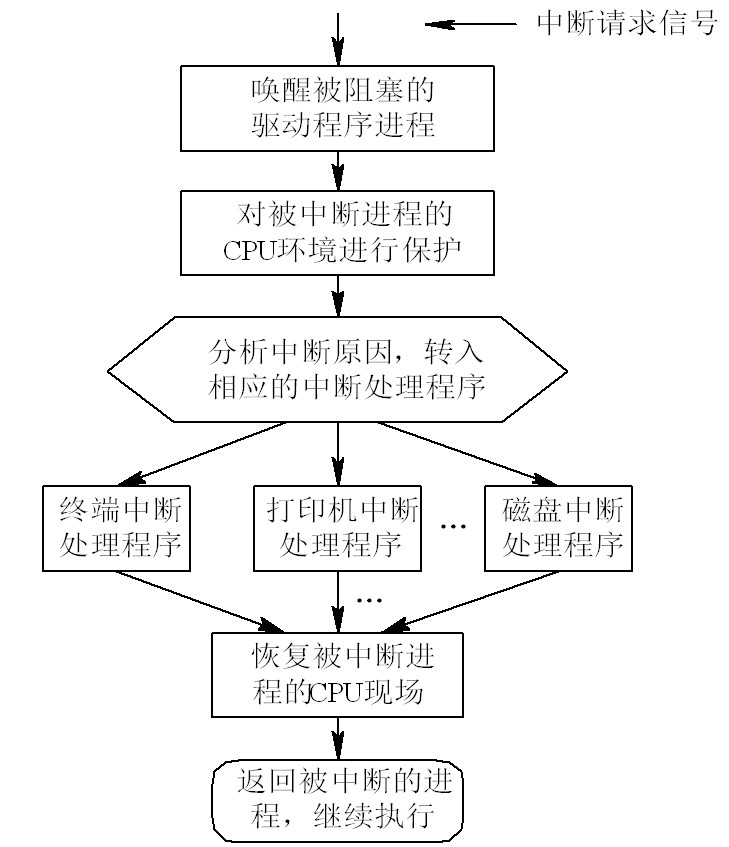
\includegraphics[width=0.5\textwidth]{figure/dev-int-process.jpg}
  \end{center}
\end{frame}

\begin{frame}[fragile]{~}
  ~
\end{frame}



\subsection{5.6 磁盘存储器管理}
\begin{frame}[fragile]{5.6 磁盘存储器管理}
  \begin{easylist}
    & 磁盘存储容量巨大,速度快,支持随机存取,因此现代计算机都配置了磁盘存储器。
    改善磁盘性能,是现代操作系统的重要任务之一。
    & 日常问题
    && 磁盘擦写次数
    && 
  \end{easylist}
\end{frame}

\note{还有就是,硬盘是可以重复擦写的。这些大家应该都知道的。但是擦写次数有限制的,
  有的朋友也不要刻意的去装系统。这样对于我们的硬盘也是不好的。也不要多格式化,尽
  量少对硬盘有读写的操作,是尽量,比如大量的复制和删除电影文件,等等一系列的类似
  操作!

  磁盘设备应包括磁盘驱动器、适配器及盘片,它们既可以作为输入设备,也可作为输出设
  备或称载体。控制软盘读和写,即输入或输出是由磁盘驱动器及其适配器来完成的,从功
  能上来说,一台磁盘设备与一台录放机的作用是相同的,一盘录音带可反复地录音, 那么
  软盘片或硬盘片,或称信息载体,也可以反复地被改写。}

\begin{frame}[fragile]{5.6 磁盘存储器管理}
  \begin{easylist}
    & 5.6.0 硬盘的发展历史
    & 5.6.1 磁盘性能简述
    & 5.6.2 磁盘调度
    & 5.6.3 磁盘高速缓存
    & 5.6.4 提高磁盘I/O速度的其他方法
    & 5.6.5 独立磁盘冗余阵列
  \end{easylist}
\end{frame}

\begin{frame}[fragile, allowframebreaks]{硬盘的发展历史}
  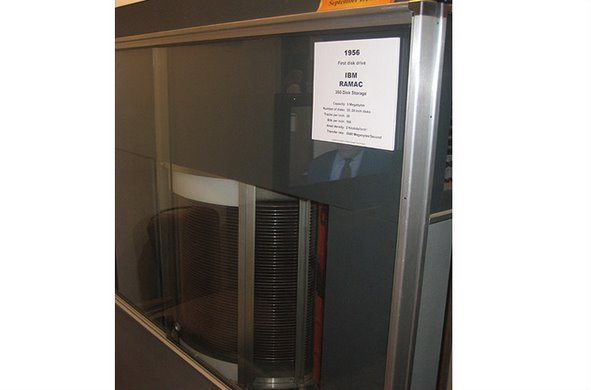
\includegraphics[width=0.7\textwidth]{figure/disk_ramac350.jpg}

  \pause

  1956年,IBM发明了第一块硬盘RAMAC 350(Random Access Method of Accounting and
  Control),支持随机读取,硬盘比冰箱大,容量是5MB

  \newpage




\end{frame}


\subsubsection{5.6.1 磁盘性能简述}
\begin{frame}[fragile]{5.6.1 磁盘性能简述}
  \begin{center}
    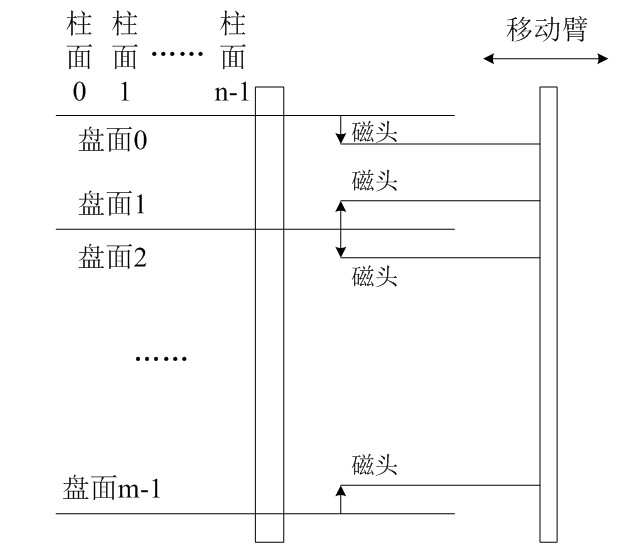
\includegraphics[width=0.45\textwidth]{figure/dev-disk.jpg}
  \end{center}
  \begin{easylist}
    & 1. 物理结构 
    && 包括一或多个盘片,每个盘片分两面
    && 每个盘面分若干磁道,各盘面上序号相同的磁道构成一个柱面
  \end{easylist}
\end{frame}


\begin{frame}[fragile]{2. 磁盘格式化}
  \begin{center}
    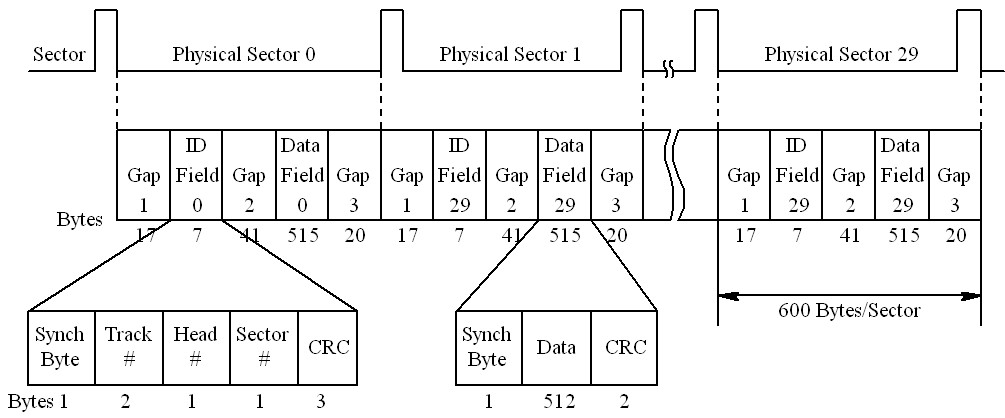
\includegraphics[width=0.85\textwidth]{figure/dev-disk-format.jpg}
  \end{center}
\end{frame}

\begin{frame}[fragile]{格式化的处理}
  \begin{easylist}
    & 格式化就是把一张空白的盘划分成一个个小的区域,并编号,供计算机储存,读取数
    据。没有这个工作的话,计算机就不知道在哪写,从哪读。
  \end{easylist}
\end{frame}

\begin{frame}[fragile]{3. 磁盘的类型}
  \begin{easylist}
    & 1) 固定头磁盘
    && 每条磁道上都有一个读写磁头,实现并行读/写,有效地提高了磁盘的I/O速度。主要用于大容量磁盘上
    & 2)移动头磁盘
    && 每个盘面配有一个磁头,为访问磁盘上的所有磁道,磁头必须能移动以寻道。
    && 串行方式读/写,致使其I/O速度较慢
    && 结构简单,广泛应用于中小型磁盘设备中
  \end{easylist}
\end{frame}

\begin{frame}[fragile]{4. 磁盘访问时间 I}
  \begin{easylist}
    & 寻道时间+旋转延迟时间+传输时间
    & 1) 寻道时间$T_s$ (seek time)
    && 这是指把磁臂(磁头)移动到指定磁道上所经历的时间。该时间是启动磁臂的时间s与
    磁头移动n条磁道所花费的时间之和, 即
    $$T_s = m \times n + s$$
    && 其中,m是一常数,与磁盘驱动器的速度有关,对一般磁盘, m=0.2;对高速磁
    盘,$m \leq 0.1$m,磁臂的启动时间约为2 ms。 这样,对一般的温盘, 其寻道时间将
    随寻道距离的增加而增大, 大体上是5--30 ms。
  \end{easylist}
\end{frame}

\begin{frame}[fragile]{4. 磁盘访问时间 II}
  \begin{easylist}
    & 2) 旋转延迟时间$T_r$ (rotational delay)
    && 这是指定扇区移动到磁头下面所经历的时间
    && 平均旋转延迟时间:
    $$E(T_r)=\dfrac{1}{2r}$$
    && $r$:磁盘转速
    \vspace{1cm}
    && 典型的旋转速度为5400r/min,即每转需要11.1ms,平均旋转延迟为5.55ms
  \end{easylist}
\end{frame}

\begin{frame}[fragile]{4. 磁盘访问时间 III}
  \begin{easylist}
  & 3) 传输时间$T_t$ (transfer time)
  && 这是指把数据从磁盘读出或向磁盘写入数据所经历的时间。Tt的大小与每次所读/写的字节数b和旋转速度有关: 
  $$T_t = \dfrac{b}{rN}$$
  && 其中,r为磁盘每秒钟的转数;N为一条磁道上的字节数, 当一次读/写的字节数相当
  于半条磁道上的字节数时,$T_t$与$T_r$相同
  \end{easylist}
\end{frame}

\begin{frame}[fragile]{例子}
  \begin{easylist}
    & 由于特定磁盘,只有集中放数据,集中读写(读写字节数b大)才能更好提高传输效率,例:
    && 寻道时间: 20ms
    && 磁盘通道传输速率: 1MB/s
    && 转速r=3600rpm
    && 每扇区512字节
    && 每磁道32 扇区
    && 目标:读 128k 数据
  \end{easylist}
\end{frame}

\begin{frame}[fragile]{Question}
  \begin{easylist}
    & 每转所需要的时间是多少?
    & 计算平均旋转延迟时间?
    & 每一条磁道上的字节数是多少?
    & 读取每个扇区数据的传输时间为多少?
    & 128K数据需要存放多少个扇区?
    & 128K数据需要存放多少个磁道?
  \end{easylist}
\end{frame}

\begin{frame}[fragile]{Answer}
  \begin{easylist}
    & 每转所需要的时间为:60*1000/3600=16.7ms
    & 平均旋转延迟时间为:60*1000/3600/2=8.3ms
    & 一条磁道上的字节数为:512*32=16384字节,即16K
    & 读取每个扇区数据的传输时间:0.5K/16K*(每转的时间)=(1/32)*(60*1000/3600)ms=0.521ms
    & 128K数据需要存放多少个扇区:128/(512/1024)=256
    & 128K数据需要存放多少个磁道:256/32=8
  \end{easylist}
\end{frame}

\begin{frame}[fragile]{时间比较}
  \begin{easylist}
    & 顺序组织
    && 20+(8.3+16.7)×8=220(ms)
    & 随机组织
    && (20+8.3+0.5)×256=7373(ms)
  \end{easylist}
\end{frame}


\begin{frame}[fragile]{磁盘交叉编址}
  \begin{center}
    \scalebox{1.0}{
      \begin{tikzpicture}[scale=1]
        \draw[thin,fill=yellow!5] (0,0) circle (1.5cm) ;
	\draw[] (-1.5,0) -- (1.5,0) (0,-1.5)--(0,1.5);
	\draw[] (225:1.5)--(45:1.5) (-45:1.5)--(135:1.5);
	\draw node at(20:1) {1} node at(65:1) {0} node at(110:1) {7}
        node at(155:1){6} node at(200:1){5} node at(245:1){4}
	node at (290:1){3} node at (335:1){2};
	\draw node at (-90:2) {无交叉编址};
      \end{tikzpicture} \hspace{0.2cm}
      \begin{tikzpicture}[scale=1]
        \draw[thin,fill=blue!5] (0,0) circle (1.5cm) ;
	\draw[] (-1.5,0) -- (1.5,0) (0,-1.5)--(0,1.5);
	\draw[] (225:1.5)--(45:1.5) (-45:1.5)--(135:1.5);
	\draw node at(20:1) {4} node at(65:1) {0} node at(110:1) {7}
        node at(155:1){3} node at(200:1){6} node at(245:1){2}
	node at (290:1){5} node at (335:1){1};
	\draw node at (-90:2) {单交叉编址};
      \end{tikzpicture} \hspace{0.2cm}
      \begin{tikzpicture}[]
        \draw[thin,fill=red!5] (0,0) circle (1.5cm) ;
	\draw[] (-1.5,0) -- (1.5,0) (0,-1.5)--(0,1.5);
	\draw[] (225:1.5)--(45:1.5) (-45:1.5)--(135:1.5);
	\draw node at(20:1) {3} node at(65:1) {0} node at(110:1) {5}
        node at(155:1){2} node at(200:1){7} node at(245:1){4}
	node at (290:1){1} node at (335:1){6};
	\draw node at (-90:2) {双交叉编址};
      \end{tikzpicture}
    }
  \end{center}
\end{frame}


\begin{frame}[fragile]{练习}
  \begin{easylist}
    & 假定磁盘转速为20ms/圈,磁盘格式化时每个磁道被划分成10个扇区,今有10个逻辑记
    录(每个记录的大小刚好和扇区的大小相等)存放在同一磁道上,处理程序每次从磁盘
    读出一个记录后要花4ms进行处理,现要求顺序处理这10个记录,若磁头现在正处在首个
    逻辑记录的始点位置,请问:

    && 1. 按逆时针方向安排10个逻辑记录(磁盘顺时针方向转),处理程序处理完这10个
    记录所花费的时间是多少?%6+9×(12+6)=168

    && 2. 按最优化分布重新安排这10个逻辑记录,写出记录的安排,并计算出所需要处理
    的时间。
  \end{easylist}
\end{frame}


\subsubsection{5.6.2 磁盘调度 }

\begin{frame}[fragile]{5.6.2 磁盘调度 }
  \begin{block}{目标:减少寻道时间}
    在多道程序环境下,OS为每个I/O设备维护一条请求队列,对一个磁盘,队列中可能有来
    自多个进程的许多I/O请求,如果随机地从队列中选择一个进程,则磁道访问完全随机,
    性能很差,因此需要更好的调度策略。
  \end{block}
\end{frame}


\begin{frame}[fragile]{5.6.2 磁盘调度 }
  \begin{easylist}
    & 一、FCFS(Fisrt Come, First Served)
    && 也可以称为FIFO
    && 特点:简单,寻道时间长,相当于随机访问模式。
    && 另一种较好的调度策略---LIFO
    & 二、SSTF(最短寻道优先)
  \end{easylist}
  \begin{block}{练习}
    假设当前时刻先后需要访问的磁道编号分别为:55, 58, 39, 18, 90, 160, 150, 38,
    184,假设磁头位于磁道100位置 \\ 分别计算FCFS和SSTF的平均寻道长度
  \end{block}
\end{frame}


\begin{frame}[fragile]{FSFS vs. SSTF}
  \begin{columns}[onlytextwidth,T]
    \begin{column}{0.45\textwidth}
      \begin{table}
        \caption{FCFS调度算法}
        \begin{tabular}{|c|c|}
          \hline
          下一个访问磁道 & 移动距离 \\ \hline
          55 & 45\\ \hline
          58 & 3\\ \hline
          39 & 19\\ \hline
          18 & 21\\ \hline
          90 & 72\\ \hline
          160 & 70\\ \hline
          150 & 10\\ \hline
          38 & 112\\ \hline
          184 & 146\\ \hline
        \end{tabular}
      \end{table}

      平均寻道长度:55.3
    \end{column}
    \begin{column}{0.45\textwidth}
      \begin{table}
        \caption{SSTF调度算法}
        \begin{tabular}{|c|c|}
          \hline
          下一个访问磁道 & 移动距离 \\ \hline
          90 & 10 \\ \hline
          58 & 32 \\ \hline
          55 & 3 \\ \hline
          39 & 16 \\ \hline
          38 & 1 \\ \hline
          18 & 20 \\ \hline
          150 & 132 \\ \hline
          160 & 10 \\ \hline
          184 & 24 \\ \hline
        \end{tabular}
      \end{table}

      平均寻道长度:27.5
    \end{column}
  \end{columns}

  假设均从100磁道开始.
\end{frame}


\begin{frame}[fragile]{5.6.2 磁盘调度 - cont.}
  \begin{easylist}
    & 三、扫描算法。
    && 1.进程“饥饿现象”
    &&& SSTF存在。
    && 2.SCAN算法(电梯调度算法):
    &&& 在移动方向固定的情况下采用了SSTF,以避免饥饿现象 
  \end{easylist}
\end{frame}

\begin{frame}[fragile]{5.6.2 磁盘调度 - cont.}
  \begin{easylist}
    & 四、循环扫描CSCAN(图9-5)
    && 一个方向读完,不是象SCAN那样回头,而是循环。
    && 最迟访问时间:2T xx T+Smax
    & 五、N—Step—SCAN和FSCAN算法。
    && 1. N—Step—SCAN
    &&& 粘臂:由于连续对某磁道访问引起的垄断访问,将磁盘请求队列分为长为N的子队
    列m个,如下图处理。当N=1时,为FCFS。当N取值很大时,为SCAN.
  \end{easylist}

  \begin{center}
    \begin{tikzpicture}[c/.style={draw, minimum height=0.5cm, minimum width=0.8cm}]
      \coordinate (b11) at (0,0);
      \foreach \line in {1,2,m}{
        \draw[] node[c, below=0.35 of b11] (b11) {} node[c, right=0 of b11] (b12) {}  node[c, right=0 of b12] (b13) {}  node[c, right=0 of b13] (b14) {}  node[c, right=0 of b14, minimum width=2cm] (b15) {$\cdots$}  node[c, right=0 of b15] (b16) {$n$} node[left=0.5 of b11]{\line};
      };

      \path[->, thick] (6.5,-0.5) edge node[rotate=-90, yshift=0.5cm]{FCFS} ++(0,-2);
    \end{tikzpicture}
  \end{center}
\end{frame}

\begin{frame}[fragile]{5.6.2 磁盘调度 - cont.}
  \begin{easylist}
    && 2. FSCAN 
  \end{easylist}

  \begin{center}
    \begin{tikzpicture}[c/.style={draw, minimum height=0.5cm, minimum width=0.8cm}]
      \draw[] node[c] (b11) {} node[c, right=0 of b11] (b12) {}  node[c, right=0 of b12] (b13) {}  node[c, right=0 of b13] (b14) {}  node[c, right=0 of b14, minimum width=2cm] (b15) {$\cdots$}  node[c, right=0 of b15] (b16) {$n$} node[left=0.5 of b11]{当前请求队列};
      \draw[] node[c, below=of b11] (b21) {} node[c, right=0 of b21] (b22) {}  node[c, right=0 of b22] (b23) {}  node[c, right=0 of b23] (b24) {}  node[c, right=0 of b24, minimum width=2cm] (b25) {$\cdots$}  node[c, right=0 of b25] (b26) {$n$} node[left=0.5 of b21]{新请求队列};

      \path[->, thick] ($(b21.south) + (0,-0.5)$) edge node[below]{SCAN} ($(b26.south) + (0,-0.5)$);
      \path[->, thick] (6.5,0.2) edge node[rotate=-90, yshift=0.5cm]{FCFS} ++(0,-2);
    \end{tikzpicture}
  \end{center}
\end{frame}


\begin{frame}[fragile]{FSFS vs. SSTF}
  \begin{easylist}
    & 假设当前时刻先后需要访问的磁道编号分别为:55,58,39,18,90,160,150,38,184,
    假设磁头位于磁道100位置
    && 分别计算SCAN和CSCAN的平均寻道长度(磁头向增加方向移动)
  \end{easylist}
\end{frame}


\begin{frame}[fragile]{SCAN vs. CSCAN}
  \begin{columns}[onlytextwidth,T]
    \begin{column}{0.45\textwidth}
      \begin{table}
        \caption{SCAN调度算法}
        \begin{tabular}{|c|c|}
          \hline
          下一个访问磁道 & 移动距离 \\ \hline
          150 & 50\\ \hline
          160 & 10\\ \hline
          184 & 24\\ \hline
          90 & 94\\ \hline
          58 & 32\\ \hline
          55 & 3\\ \hline
          39 & 16\\ \hline
          38 & 1\\ \hline
          18 & 20\\ \hline
        \end{tabular}
      \end{table}

      平均寻道长度:27.8
    \end{column}
    \begin{column}{0.45\textwidth}
      \begin{table}
        \caption{CSCAN调度算法}
        \begin{tabular}{|c|c|}
          \hline
          下一个访问磁道 & 移动距离 \\ \hline
          150 & 50 \\ \hline
          160 & 10 \\ \hline
          184 & 24 \\ \hline
          18 & 166 \\ \hline
          38 & 20 \\ \hline
          39 & 1 \\ \hline
          55 & 16 \\ \hline
          58 & 3 \\ \hline
          90 & 32 \\ \hline
        \end{tabular}
      \end{table}

      平均寻道长度:35.8
    \end{column}
  \end{columns}
\end{frame}


\subsubsection{5.6.3 磁盘高速缓存}
\begin{frame}[fragile, allowframebreaks]{5.6.3 磁盘高速缓存}
  \begin{easylist}
    & 形式
    && 逻辑上是磁盘、物理上是驻留在内存中的盘块
    && 固定大小和可变大小
    & 数据交付方式
    && 数据交付指将磁盘高速缓存中的数据传送给请求者进程
    && 步骤:先查缓存、后查磁盘并更新缓存
    && 方式:
    &&& 数据交付
    &&& 指针交付:只指向高速缓存中某区域的指针

    \newpage

    & 置换算法
    && 最近最久
    && 访问频率
    && 可预见性
    && 数据一致性:将需要一致性的块放在替换队列的头部,优先回写。
    & 周期性回写磁盘
    && 例:
    &&& Unix周期性调用SYNC
    &&& ms-dos采用写穿透方式
  \end{easylist}
\end{frame}


\subsubsection{5.6.4 提高磁盘I/O速度的其它方法}
\begin{frame}[fragile]{5.6.4 提高磁盘I/O速度的其它方法}
  \begin{easylist}
    & 提前读
    & 延迟写
    && 访问频率高的磁盘块放在替换队列的尾部,减少回写次数
    & 优化物理块的分布
    && 目的是减小磁头移动距离
    && 簇分配方式:一个簇为多个连续的块
    & 虚拟盘(RAM盘)
    && 和磁盘高速缓存区别:虚拟盘由用户控制;磁盘高速缓存由系统控制。
  \end{easylist}
\end{frame}

\subsubsection{5.6.5 独立磁盘冗余阵列}
\begin{frame}[fragile]{5.6.5 独立磁盘冗余阵列}
  \begin{easylist}
    & 辅存性能的提高速度远远低于处理器和内存的提高速度,使得磁盘存储系统称为提高
    计算机整体性能的主要问题
    & 如单个组件性能提升有限,可采用多个组件并行的方式
    & 加州大学伯克利分校的研究小组于1988年首次提出RAID术语
    && Redundant Array of Independent Disks: 独立磁盘冗余阵列
    & 思路
    && RAID是一组物理磁盘驱动器,OS把他们看做是一个单独的逻辑驱动器
    && 数据分布在物理驱动器阵列中
    && 使用冗余的磁盘容量保存校验信息,从而保证当一个磁盘失效时,数据具有可恢复
    性。
    & RAID共有7个级别,从0到6,这些级别并不隐含一种层次关系
  \end{easylist}
\end{frame}

\begin{frame}[fragile]{RAID的特点}
  \begin{easylist}
    & 并行交叉存取(条化存取)
    & 冗余存取
    & 校验存取
    & 优点
    && 可靠性高
    && 磁盘I/O速度高
    && 性价比高
  \end{easylist}
\end{frame}

\begin{frame}[fragile]{RAID5}
  \begin{easylist}
    & 容错性:有 冗余类型:奇偶校验
    & 热备盘选项:有 读性能:高
    & 随机写性能:低 连续写性能:低
    & 需要的磁盘数:三个或更多
    & 可用容量:(n-1)/n的总磁盘容量(n为磁盘数)
    & 典型应用:随机数据传输要求安全性高,如金融、税务等。 
  \end{easylist}
\end{frame}


\begin{frame}[fragile]{本章实验}
  \begin{easylist}
    & 调查:硬盘的发展历史
    & 实现SSTF算法和SCAN算法
    && 要求
    &&& 给出任意的输入流、计算平均寻道长度。
    &&& 输入流长度、磁头移动方向可定制。
    &&& 测试:设有100各磁道,访问序列如下:
    &&&& 23,5,98, 14,66,25,78,34,66,74,56,87,12,39,71,49,58
    &&&& 当前磁头在50道,上次访问的磁道是18道,SCAN算法由内到外移动
  \end{easylist}
\end{frame}

\begin{frame}
  \begin{center}
    \Huge END
  \end{center}
\end{frame}
